% Camera-ready: CL4FMAgents @ NeurIPS 2026 (accepted September 29;
% camera-ready due October 10, time and timezone unspecified; regular track,
% 8 pages excluding references and appendix, non-archival).
%
% The workshop names no template on its site, its CFP, or its OpenReview
% form (site checked again 2026-10-04), so the NeurIPS 2026 style is the
% conservative default. It is vendored next to this file; without it the
% draft falls back to plain article so it always builds.
%
% Every numeric claim resolves through a macro defined in numbers.tex, which is
% generated by scripts/export_paper_numbers.py from the committed JSON
% artifacts. Do not type a number into this file. The one exception is the
% drift schedule in Section 2, which is a configuration constant rather than an
% analysis result; tests/test_paper_drift_description.py holds it to the
% configs, because it had already drifted once.

\newif\ifusevenue
\IfFileExists{neurips_2026.sty}{\usevenuetrue}{\usevenuefalse}

\ifusevenue
  \documentclass{article}
  \usepackage[final]{neurips_2026}
  \makeatletter
  \renewcommand{\@noticestring}{NeurIPS 2026 Workshop on
    Continual Learning in the Era of Foundation Models and Embodied Agents
    (CL4FMAgents).}
  \makeatother
\else
  \documentclass[10pt]{article}
  \usepackage[letterpaper,margin=1.1in]{geometry}
  \usepackage{times}
\fi

% tectonic compiles under XeTeX, where the style's NFSS \rmdefault{ptm} has no
% TU font definitions and bold/italic silently fall back to regular Latin
% Modern. T1 fontenc restores a real Times-family face with all shapes.
\usepackage[T1]{fontenc}
\usepackage{amsmath}
\usepackage{amssymb}
\usepackage{booktabs}
\usepackage{graphicx}
\usepackage{microtype}
\usepackage{url}
\usepackage[hidelinks]{hyperref}
\ifusevenue\else
  \usepackage[round]{natbib}
\fi

% Generated by scripts/export_paper_numbers.py -- do not edit by hand.
% Every numeric claim in the manuscript resolves through these macros.

\newcommand{\ActorFrequency}{2}
\newcommand{\ActorLR}{0.0003}
\newcommand{\AdjSepAnt}{0}
\newcommand{\AdjSepHalfcheetah}{0}
\newcommand{\AdjSepHopper}{0}
\newcommand{\AdjSepPcgym}{0}
\newcommand{\AdjSepWalkerTwod}{0}
\newcommand{\AdjTotAnt}{7}
\newcommand{\AdjTotHalfcheetah}{7}
\newcommand{\AdjTotHopper}{7}
\newcommand{\AdjTotPcgym}{7}
\newcommand{\AdjTotWalkerTwod}{7}
\newcommand{\AdjacentExploratory}{2}
\newcommand{\AdjacentHolmCutoff}{0.001786}
\newcommand{\AdjacentPFloor}{0.001953}
\newcommand{\AdjacentSeparated}{0}
\newcommand{\AdjacentTotal}{35}
\newcommand{\AllPolicyPairs}{28}
\newcommand{\Alpha}{0.05}
\newcommand{\BestAnt}{RecencyWeighted}
\newcommand{\BestHalfcheetah}{RecencyWeighted}
\newcommand{\BestHiAnt}{747.0}
\newcommand{\BestHiHalfcheetah}{4392.9}
\newcommand{\BestHiHopper}{1008.3}
\newcommand{\BestHiPcgym}{-360.0}
\newcommand{\BestHiWalkerTwod}{612.5}
\newcommand{\BestHopper}{RecentOnly}
\newcommand{\BestIqmAnt}{649.9}
\newcommand{\BestIqmHalfcheetah}{3897.8}
\newcommand{\BestIqmHopper}{807.9}
\newcommand{\BestIqmPcgym}{-695.5}
\newcommand{\BestIqmWalkerTwod}{507.3}
\newcommand{\BestLoAnt}{582.3}
\newcommand{\BestLoHalfcheetah}{3619.9}
\newcommand{\BestLoHopper}{667.2}
\newcommand{\BestLoPcgym}{-1195.8}
\newcommand{\BestLoWalkerTwod}{438.6}
\newcommand{\BestPcgym}{RecencyWeighted}
\newcommand{\BestWalkerTwod}{RecentOnly}
\newcommand{\BudgetExactAnt}{yes}
\newcommand{\BudgetExactHalfcheetah}{yes}
\newcommand{\BudgetExactHopper}{yes}
\newcommand{\BudgetExactPcgym}{yes}
\newcommand{\BudgetExactWalkerTwod}{yes}
\newcommand{\CalBiasheteroscedasticconcordant}{-0.000}
\newcommand{\CalBiasheteroscedasticpartialreversal}{-0.002}
\newcommand{\CalBiasheteroscedasticunequalconcordant}{0.028}
\newcommand{\CalBiashomoscedasticconcordant}{-0.010}
\newcommand{\CalCovheteroscedasticconcordant}{0.960}
\newcommand{\CalCovheteroscedasticpartialreversal}{0.930}
\newcommand{\CalCovheteroscedasticunequalconcordant}{0.960}
\newcommand{\CalCovhomoscedasticconcordant}{0.978}
\newcommand{\CalRejectheteroscedasticconcordant}{0.030}
\newcommand{\CalRejectheteroscedasticpartialreversal}{0.390}
\newcommand{\CalRejectheteroscedasticunequalconcordant}{0.050}
\newcommand{\CalRejecthomoscedasticconcordant}{0.005}
\newcommand{\CalibrationCases}{4}
\newcommand{\CalibrationCoverageEqual}{0.978}
\newcommand{\CalibrationCoverageHetero}{0.960}
\newcommand{\CalibrationCoverageReversal}{0.930}
\newcommand{\CalibrationCoverageUnequal}{0.960}
\newcommand{\CalibrationDatasets}{400}
\newcommand{\CalibrationHalf}{5}
\newcommand{\CalibrationNoiseRatio}{3.4}
\newcommand{\CalibrationPolicies}{8}
\newcommand{\CalibrationPopulationDraws}{100{,}000}
\newcommand{\CalibrationPopulationSE}{0.0003}
\newcommand{\CalibrationPopulationTarget}{0.0879}
\newcommand{\CalibrationRejectionEqual}{0.005}
\newcommand{\CalibrationRejectionHetero}{0.030}
\newcommand{\CalibrationRejectionReversal}{0.390}
\newcommand{\CalibrationRejectionUnequal}{0.050}
\newcommand{\CalibrationSeeds}{10}
\newcommand{\CalibrationSigma}{0.35}
\newcommand{\CalibrationSigmaHigh}{2.5}
\newcommand{\CalibrationSigmaLow}{0.25}
\newcommand{\ChanceExpected}{1.2}
\newcommand{\CheapestAnt}{StaticMix}
\newcommand{\CheapestHalfcheetah}{RecentOnly}
\newcommand{\CheapestHopper}{RecentOnly}
\newcommand{\CheapestPcgym}{RecentOnly}
\newcommand{\CheapestWalkerTwod}{RecentOnly}
\newcommand{\ContrastAnt}{23.9}
\newcommand{\ContrastBH}{2}
\newcommand{\ContrastBHList}{HalfCheetah, Hopper}
\newcommand{\ContrastDAnt}{0.56}
\newcommand{\ContrastDHalfcheetah}{3.19}
\newcommand{\ContrastDHopper}{1.04}
\newcommand{\ContrastDPcgym}{1.38}
\newcommand{\ContrastDWalkerTwod}{0.72}
\newcommand{\ContrastHalfcheetah}{459.2}
\newcommand{\ContrastHiAnt}{46.3}
\newcommand{\ContrastHiHalfcheetah}{546.1}
\newcommand{\ContrastHiHopper}{201.6}
\newcommand{\ContrastHiPcgym}{176.2}
\newcommand{\ContrastHiWalkerTwod}{83.1}
\newcommand{\ContrastHolm}{1}
\newcommand{\ContrastHolmList}{HalfCheetah}
\newcommand{\ContrastHopper}{132.5}
\newcommand{\ContrastLoAnt}{-3.0}
\newcommand{\ContrastLoHalfcheetah}{376.1}
\newcommand{\ContrastLoHopper}{52.7}
\newcommand{\ContrastLoPcgym}{43.0}
\newcommand{\ContrastLoWalkerTwod}{9.4}
\newcommand{\ContrastNTests}{5}
\newcommand{\ContrastPAnt}{0.1094}
\newcommand{\ContrastPFloorAnt}{0.0020}
\newcommand{\ContrastPFloorHalfcheetah}{0.0020}
\newcommand{\ContrastPFloorHopper}{0.0020}
\newcommand{\ContrastPFloorPcgym}{0.0625}
\newcommand{\ContrastPFloorWalkerTwod}{0.0020}
\newcommand{\ContrastPHalfcheetah}{0.0020}
\newcommand{\ContrastPHopper}{0.0156}
\newcommand{\ContrastPPcgym}{0.1250}
\newcommand{\ContrastPWalkerTwod}{0.0469}
\newcommand{\ContrastPcgym}{118.7}
\newcommand{\ContrastResolvedAnt}{no}
\newcommand{\ContrastResolvedHalfcheetah}{yes}
\newcommand{\ContrastResolvedHopper}{yes}
\newcommand{\ContrastResolvedPcgym}{yes}
\newcommand{\ContrastResolvedWalkerTwod}{yes}
\newcommand{\ContrastSignsAnt}{8}
\newcommand{\ContrastSignsHalfcheetah}{10}
\newcommand{\ContrastSignsHopper}{8}
\newcommand{\ContrastSignsPcgym}{4}
\newcommand{\ContrastSignsWalkerTwod}{8}
\newcommand{\ContrastUncorrected}{4}
\newcommand{\ContrastWalkerTwod}{45.0}
\newcommand{\CriticLR}{0.0003}
\newcommand{\CrossAntForgImp}{0.333}
\newcommand{\CrossAntRecForg}{0.377}
\newcommand{\CrossAntRecImp}{0.238}
\newcommand{\CrossAntRetForg}{0.336}
\newcommand{\CrossAntRetImp}{0.216}
\newcommand{\CrossAntRetRec}{0.275}
\newcommand{\CrossHalfcheetahForgImp}{0.253}
\newcommand{\CrossHalfcheetahRecForg}{0.410}
\newcommand{\CrossHalfcheetahRecImp}{0.222}
\newcommand{\CrossHalfcheetahRetForg}{0.247}
\newcommand{\CrossHalfcheetahRetImp}{0.047}
\newcommand{\CrossHalfcheetahRetRec}{0.218}
\newcommand{\CrossHopperForgImp}{0.645}
\newcommand{\CrossHopperRecForg}{0.427}
\newcommand{\CrossHopperRecImp}{0.541}
\newcommand{\CrossHopperRetForg}{0.635}
\newcommand{\CrossHopperRetImp}{0.325}
\newcommand{\CrossHopperRetRec}{0.534}
\newcommand{\CrossWalkerTwodForgImp}{0.614}
\newcommand{\CrossWalkerTwodRecForg}{0.423}
\newcommand{\CrossWalkerTwodRecImp}{0.535}
\newcommand{\CrossWalkerTwodRetForg}{0.627}
\newcommand{\CrossWalkerTwodRetImp}{0.329}
\newcommand{\CrossWalkerTwodRetRec}{0.531}
\newcommand{\DropFlagDescriptions}{Hopper (return versus forgetting), HalfCheetah (recovery versus forgetting)}
\newcommand{\DropMetric}{budget-normalised improvement}
\newcommand{\DropSurvA}{return}
\newcommand{\DropSurvB}{forgetting}
\newcommand{\DropSurvEnv}{Hopper}
\newcommand{\EvalSeedOffset}{10{,}000}
\newcommand{\EvaluationEpisodes}{3}
\newcommand{\ExHiAntForgImp}{0.066}
\newcommand{\ExHiAntRecForg}{0.061}
\newcommand{\ExHiAntRecImp}{0.031}
\newcommand{\ExHiAntRetForg}{0.045}
\newcommand{\ExHiAntRetImp}{0.051}
\newcommand{\ExHiAntRetRec}{0.031}
\newcommand{\ExHiHalfcheetahForgImp}{0.053}
\newcommand{\ExHiHalfcheetahRecForg}{0.150}
\newcommand{\ExHiHalfcheetahRecImp}{0.024}
\newcommand{\ExHiHalfcheetahRetForg}{0.058}
\newcommand{\ExHiHalfcheetahRetImp}{0.025}
\newcommand{\ExHiHalfcheetahRetRec}{0.036}
\newcommand{\ExHiHopperForgImp}{0.428}
\newcommand{\ExHiHopperRecForg}{0.041}
\newcommand{\ExHiHopperRecImp}{0.357}
\newcommand{\ExHiHopperRetForg}{0.395}
\newcommand{\ExHiHopperRetImp}{0.111}
\newcommand{\ExHiHopperRetRec}{0.368}
\newcommand{\ExHiWalkerTwodForgImp}{0.479}
\newcommand{\ExHiWalkerTwodRecForg}{0.062}
\newcommand{\ExHiWalkerTwodRecImp}{0.335}
\newcommand{\ExHiWalkerTwodRetForg}{0.492}
\newcommand{\ExHiWalkerTwodRetImp}{0.101}
\newcommand{\ExHiWalkerTwodRetRec}{0.325}
\newcommand{\ExLoAntForgImp}{-0.167}
\newcommand{\ExLoAntRecForg}{-0.069}
\newcommand{\ExLoAntRecImp}{-0.055}
\newcommand{\ExLoAntRetForg}{-0.159}
\newcommand{\ExLoAntRetImp}{-0.019}
\newcommand{\ExLoAntRetRec}{-0.028}
\newcommand{\ExLoHalfcheetahForgImp}{-0.153}
\newcommand{\ExLoHalfcheetahRecForg}{0.029}
\newcommand{\ExLoHalfcheetahRecImp}{-0.098}
\newcommand{\ExLoHalfcheetahRetForg}{-0.165}
\newcommand{\ExLoHalfcheetahRetImp}{-0.021}
\newcommand{\ExLoHalfcheetahRetRec}{-0.107}
\newcommand{\ExLoHopperForgImp}{0.131}
\newcommand{\ExLoHopperRecForg}{-0.079}
\newcommand{\ExLoHopperRecImp}{-0.184}
\newcommand{\ExLoHopperRetForg}{0.140}
\newcommand{\ExLoHopperRetImp}{-0.036}
\newcommand{\ExLoHopperRetRec}{-0.225}
\newcommand{\ExLoWalkerTwodForgImp}{-0.055}
\newcommand{\ExLoWalkerTwodRecForg}{-0.027}
\newcommand{\ExLoWalkerTwodRecImp}{-0.031}
\newcommand{\ExLoWalkerTwodRetForg}{0.007}
\newcommand{\ExLoWalkerTwodRetImp}{-0.037}
\newcommand{\ExLoWalkerTwodRetRec}{-0.005}
\newcommand{\ExcessAntForgImp}{-0.051}
\newcommand{\ExcessAntRecForg}{-0.004}
\newcommand{\ExcessAntRecImp}{-0.012}
\newcommand{\ExcessAntRetForg}{-0.057}
\newcommand{\ExcessAntRetImp}{0.016}
\newcommand{\ExcessAntRetRec}{0.002}
\newcommand{\ExcessHalfcheetahForgImp}{-0.050}
\newcommand{\ExcessHalfcheetahRecForg}{0.090}
\newcommand{\ExcessHalfcheetahRecImp}{-0.037}
\newcommand{\ExcessHalfcheetahRetForg}{-0.054}
\newcommand{\ExcessHalfcheetahRetImp}{0.002}
\newcommand{\ExcessHalfcheetahRetRec}{-0.035}
\newcommand{\ExcessHopperForgImp}{0.279}
\newcommand{\ExcessHopperRecForg}{-0.019}
\newcommand{\ExcessHopperRecImp}{0.086}
\newcommand{\ExcessHopperRetForg}{0.267}
\newcommand{\ExcessHopperRetImp}{0.037}
\newcommand{\ExcessHopperRetRec}{0.072}
\newcommand{\ExcessWalkerTwodForgImp}{0.212}
\newcommand{\ExcessWalkerTwodRecForg}{0.018}
\newcommand{\ExcessWalkerTwodRecImp}{0.152}
\newcommand{\ExcessWalkerTwodRetForg}{0.250}
\newcommand{\ExcessWalkerTwodRetImp}{0.032}
\newcommand{\ExcessWalkerTwodRetRec}{0.160}
\newcommand{\ExtPairPAnt}{0.0020}
\newcommand{\ExtPairPHalfcheetah}{0.0020}
\newcommand{\ExtPairPHopper}{0.0156}
\newcommand{\ExtPairPPcgym}{0.1250}
\newcommand{\ExtPairPWalkerTwod}{0.0137}
\newcommand{\ExtremesBH}{3}
\newcommand{\ExtremesBHList}{Ant, HalfCheetah, PC-Gym}
\newcommand{\ExtremesNTests}{5}
\newcommand{\ExtremesPairedBH}{4}
\newcommand{\FloorAntForgImp}{0.383}
\newcommand{\FloorAntRecForg}{0.380}
\newcommand{\FloorAntRecImp}{0.250}
\newcommand{\FloorAntRetForg}{0.393}
\newcommand{\FloorAntRetImp}{0.200}
\newcommand{\FloorAntRetRec}{0.274}
\newcommand{\FloorEnv}{Hopper}
\newcommand{\FloorFullForg}{0.253}
\newcommand{\FloorFullImp}{0.261}
\newcommand{\FloorFullRec}{0.510}
\newcommand{\FloorFullRet}{0.308}
\newcommand{\FloorHalfForg}{0.449}
\newcommand{\FloorHalfImp}{0.426}
\newcommand{\FloorHalfRec}{0.561}
\newcommand{\FloorHalfRet}{0.413}
\newcommand{\FloorHalfcheetahForgImp}{0.303}
\newcommand{\FloorHalfcheetahRecForg}{0.320}
\newcommand{\FloorHalfcheetahRecImp}{0.259}
\newcommand{\FloorHalfcheetahRetForg}{0.301}
\newcommand{\FloorHalfcheetahRetImp}{0.045}
\newcommand{\FloorHalfcheetahRetRec}{0.253}
\newcommand{\FloorHopperForgImp}{0.366}
\newcommand{\FloorHopperRecForg}{0.446}
\newcommand{\FloorHopperRecImp}{0.454}
\newcommand{\FloorHopperRetForg}{0.368}
\newcommand{\FloorHopperRetImp}{0.288}
\newcommand{\FloorHopperRetRec}{0.462}
\newcommand{\FloorWalkerTwodForgImp}{0.402}
\newcommand{\FloorWalkerTwodRecForg}{0.406}
\newcommand{\FloorWalkerTwodRecImp}{0.383}
\newcommand{\FloorWalkerTwodRetForg}{0.377}
\newcommand{\FloorWalkerTwodRetImp}{0.297}
\newcommand{\FloorWalkerTwodRetRec}{0.371}
\newcommand{\FloorWorstMetric}{recovery}
\newcommand{\FloorWorstValue}{0.510}
\newcommand{\FullSplitCount}{252}
\newcommand{\HiddenLayers}{2}
\newcommand{\HiddenWidth}{256}
\newcommand{\IccAnt}{0.375}
\newcommand{\IccHalfcheetah}{0.717}
\newcommand{\IccHopper}{0.671}
\newcommand{\IccMax}{0.91}
\newcommand{\IccMaxEnv}{PC-Gym}
\newcommand{\IccMin}{0.38}
\newcommand{\IccMinEnv}{Ant}
\newcommand{\IccPcgym}{0.912}
\newcommand{\IccWalkerTwod}{0.632}
\newcommand{\JackHalfSize}{4}
\newcommand{\JackSplitCount}{630}
\newcommand{\JointNTests}{15}
\newcommand{\JointUnchanged}{yes}
\newcommand{\LargestObservedExcess}{0.279}
\newcommand{\LearningStarts}{5{,}000}
\newcommand{\MetricFlagDescriptions}{Hopper: return versus forgetting, excess +0.267 [+0.140, +0.395]; Hopper: forgetting versus budget-normalised improvement, excess +0.279 [+0.131, +0.428]; HalfCheetah: recovery versus forgetting, excess +0.090 [+0.029, +0.150]}
\newcommand{\MetricHalfSize}{5}
\newcommand{\NBH}{3}
\newcommand{\NBHDrop}{2}
\newcommand{\NCellPairs}{672}
\newcommand{\NClamped}{24}
\newcommand{\NClampedPairs}{336}
\newcommand{\NDistinct}{12}
\newcommand{\NEnv}{5}
\newcommand{\NPolAnt}{8}
\newcommand{\NPolHalfcheetah}{8}
\newcommand{\NPolHopper}{8}
\newcommand{\NPolPcgym}{8}
\newcommand{\NPolWalkerTwod}{8}
\newcommand{\NRaw}{5}
\newcommand{\NTests}{24}
\newcommand{\NonWallAnt}{1.32}
\newcommand{\NonWallHalfcheetah}{1.36}
\newcommand{\NonWallHopper}{1.30}
\newcommand{\NonWallPcgym}{1.18}
\newcommand{\NonWallWalkerTwod}{1.40}
\newcommand{\ObservedUpdatesAnt}{45{,}000}
\newcommand{\ObservedUpdatesHalfcheetah}{45{,}000}
\newcommand{\ObservedUpdatesHopper}{35{,}000}
\newcommand{\ObservedUpdatesPcgym}{20{,}000}
\newcommand{\ObservedUpdatesWalkerTwod}{45{,}000}
\newcommand{\OmniPAnt}{0.01}
\newcommand{\OmniPHalfcheetah}{0.00}
\newcommand{\OmniPHopper}{0.24}
\newcommand{\OmniPPcgym}{0.01}
\newcommand{\OmniPWalkerTwod}{0.05}
\newcommand{\OrderResolvedAnt}{yes}
\newcommand{\OrderResolvedHalfcheetah}{yes}
\newcommand{\OrderResolvedHopper}{no}
\newcommand{\OrderResolvedPcgym}{no}
\newcommand{\OrderResolvedWalkerTwod}{no}
\newcommand{\OrderingResolved}{2}
\newcommand{\OrderingUnresolved}{3}
\newcommand{\OrdersFullyResolved}{0}
\newcommand{\PairDAnt}{0.60}
\newcommand{\PairDHalfcheetah}{1.76}
\newcommand{\PairDHopper}{0.41}
\newcommand{\PairDPcgym}{0.64}
\newcommand{\PairDWalkerTwod}{0.49}
\newcommand{\PartitionResolved}{4}
\newcommand{\PowerDFiveThreeSix}{0.95}
\newcommand{\PowerDTwoOneFour}{0.27}
\newcommand{\PowerDZeroThreeSix}{0.04}
\newcommand{\PowerDZeroZeroZero}{0.06}
\newcommand{\PowerDraws}{300}
\newcommand{\PowerEnv}{Hopper}
\newcommand{\PowerFalsePos}{0.06}
\newcommand{\PowerFullReversal}{1.00}
\newcommand{\PowerNoise}{140.58}
\newcommand{\PowerOneZeroZeroZero}{1.00}
\newcommand{\PowerReliableAt}{0.54}
\newcommand{\PowerSepDFiveThreeSix}{0.536}
\newcommand{\PowerSepDTwoOneFour}{0.214}
\newcommand{\PowerSepDZeroThreeSix}{0.036}
\newcommand{\PowerSepDZeroZeroZero}{0.000}
\newcommand{\PowerSepOneZeroZeroZero}{1.000}
\newcommand{\PowerWeakRate}{0.27}
\newcommand{\PowerWeakSep}{0.21}
\newcommand{\RatioAnt}{0.94}
\newcommand{\RatioHalfcheetah}{1.82}
\newcommand{\RatioHopper}{2.57}
\newcommand{\RatioPcgym}{2.15}
\newcommand{\RatioWalkerTwod}{1.48}
\newcommand{\RecWallAnt}{1.09}
\newcommand{\RecWallHalfcheetah}{1.10}
\newcommand{\RecWallHopper}{1.09}
\newcommand{\RecWallPcgym}{1.05}
\newcommand{\RecWallWalkerTwod}{1.12}
\newcommand{\RecentOnlyRankAnt}{8}
\newcommand{\RecentOnlyRankHalfcheetah}{2}
\newcommand{\RecentOnlyRankHopper}{1}
\newcommand{\RecentOnlyRankPcgym}{4}
\newcommand{\RecentOnlyRankWalkerTwod}{1}
\newcommand{\RevAbove}{HalfCheetah}
\newcommand{\RevBelow}{Ant}
\newcommand{\RevNTests}{5}
\newcommand{\RevSupported}{yes}
\newcommand{\RoAntD}{-1.28}
\newcommand{\RoAntMean}{-86.5}
\newcommand{\RoAntP}{0.0020}
\newcommand{\RoAntPos}{0}
\newcommand{\RoAntRank}{8}
\newcommand{\RoHalfcheetahD}{2.16}
\newcommand{\RoHalfcheetahMean}{347.6}
\newcommand{\RoHalfcheetahP}{0.0020}
\newcommand{\RoHalfcheetahPos}{10}
\newcommand{\RoHalfcheetahRank}{2}
\newcommand{\RoHopperD}{0.65}
\newcommand{\RoHopperMean}{117.2}
\newcommand{\RoHopperP}{0.0547}
\newcommand{\RoHopperPos}{8}
\newcommand{\RoHopperRank}{1}
\newcommand{\RoPcgymD}{0.72}
\newcommand{\RoPcgymMean}{75.2}
\newcommand{\RoPcgymP}{0.1875}
\newcommand{\RoPcgymPos}{4}
\newcommand{\RoPcgymRank}{4}
\newcommand{\RoWalkerTwodD}{0.62}
\newcommand{\RoWalkerTwodMean}{51.4}
\newcommand{\RoWalkerTwodP}{0.0820}
\newcommand{\RoWalkerTwodPos}{7}
\newcommand{\RoWalkerTwodRank}{1}
\newcommand{\SeedsAnt}{10}
\newcommand{\SeedsHalfcheetah}{10}
\newcommand{\SeedsHopper}{10}
\newcommand{\SeedsPcgym}{5}
\newcommand{\SeedsWalkerTwod}{10}
\newcommand{\SurvFirstA}{return}
\newcommand{\SurvFirstB}{forgetting}
\newcommand{\SurvFirstEnv}{Hopper}
\newcommand{\SurvFirstExcess}{0.267}
\newcommand{\SurvFirstHi}{0.395}
\newcommand{\SurvFirstLo}{0.140}
\newcommand{\SurvSecondA}{forgetting}
\newcommand{\SurvSecondB}{budget-normalised improvement}
\newcommand{\SurvSecondEnv}{Hopper}
\newcommand{\SurvSecondExcess}{0.279}
\newcommand{\SurvSecondHi}{0.428}
\newcommand{\SurvSecondLo}{0.131}
\newcommand{\SurvThirdA}{recovery}
\newcommand{\SurvThirdB}{forgetting}
\newcommand{\SurvThirdEnv}{HalfCheetah}
\newcommand{\SurvThirdExcess}{0.090}
\newcommand{\SurvThirdHi}{0.150}
\newcommand{\SurvThirdLo}{0.029}
\newcommand{\TargetFrequency}{1}
\newcommand{\TopOneAnt}{RecencyWeighted}
\newcommand{\TopOneHalfcheetah}{RecencyWeighted}
\newcommand{\TopOneHopper}{RecentOnly}
\newcommand{\TopOnePcgym}{RecencyWeighted}
\newcommand{\TopOneProbAnt}{0.65}
\newcommand{\TopOneProbHalfcheetah}{0.94}
\newcommand{\TopOneProbHopper}{0.49}
\newcommand{\TopOneProbMax}{0.94}
\newcommand{\TopOneProbMaxEnv}{HalfCheetah}
\newcommand{\TopOneProbMin}{0.47}
\newcommand{\TopOneProbMinEnv}{Walker2d}
\newcommand{\TopOneProbPcgym}{0.76}
\newcommand{\TopOneProbWalkerTwod}{0.47}
\newcommand{\TopOneWalkerTwod}{RecentOnly}
\newcommand{\TrainBatch}{256}
\newcommand{\TrainGamma}{0.99}
\newcommand{\TrainTau}{0.005}
\newcommand{\TrainingSeedMaxAnt}{60}
\newcommand{\TrainingSeedMaxHalfcheetah}{50}
\newcommand{\TrainingSeedMaxHopper}{30}
\newcommand{\TrainingSeedMaxPcgym}{65}
\newcommand{\TrainingSeedMaxWalkerTwod}{40}
\newcommand{\TrainingSeedMinAnt}{51}
\newcommand{\TrainingSeedMinHalfcheetah}{41}
\newcommand{\TrainingSeedMinHopper}{21}
\newcommand{\TrainingSeedMinPcgym}{61}
\newcommand{\TrainingSeedMinWalkerTwod}{31}
\newcommand{\WallSpreadAnt}{1.34}
\newcommand{\WallSpreadHalfcheetah}{1.39}
\newcommand{\WallSpreadHopper}{1.33}
\newcommand{\WallSpreadMax}{1.45}
\newcommand{\WallSpreadMin}{1.21}
\newcommand{\WallSpreadPcgym}{1.21}
\newcommand{\WallSpreadWalkerTwod}{1.45}
\newcommand{\WorstAnt}{RecentOnly}
\newcommand{\WorstHalfcheetah}{PER}
\newcommand{\WorstHiAnt}{554.2}
\newcommand{\WorstHiHalfcheetah}{3227.4}
\newcommand{\WorstHiHopper}{801.1}
\newcommand{\WorstHiPcgym}{-496.0}
\newcommand{\WorstHiWalkerTwod}{466.2}
\newcommand{\WorstHopper}{PER}
\newcommand{\WorstIqmAnt}{517.3}
\newcommand{\WorstIqmHalfcheetah}{2949.4}
\newcommand{\WorstIqmHopper}{641.2}
\newcommand{\WorstIqmPcgym}{-1044.3}
\newcommand{\WorstIqmWalkerTwod}{417.5}
\newcommand{\WorstLoAnt}{481.8}
\newcommand{\WorstLoHalfcheetah}{2782.8}
\newcommand{\WorstLoHopper}{477.8}
\newcommand{\WorstLoPcgym}{-1330.5}
\newcommand{\WorstLoWalkerTwod}{385.4}
\newcommand{\WorstPcgym}{PER}
\newcommand{\WorstWalkerTwod}{Uniform}


\newcommand{\ret}{\textsf{return}}
\newcommand{\rec}{\textsf{recovery}}
\newcommand{\forg}{\textsf{forgetting}}
\newcommand{\imp}{\textsf{improvement/1k}}

\title{What Ten Seeds Can and Cannot Resolve
About Replay Strategy Selection Under Distribution Shift}

\author{Youngmin Ko\thanks{Independent research. Current affiliation: KRAFTON.}\\
The Pennsylvania State University}
\date{}

\begin{document}
\maketitle

\begin{abstract}
Replay-strategy comparisons under non-stationarity --- a design choice every
continually adapting agent embeds --- are normally reported as a ranking over
policies, plus a claim that the ranking depends on the metric. We evaluate
\NPolHopper{} adaptation policies at a fixed update and replay-sample budget
across \NEnv{} drifting environments, with \SeedsHopper{} seeds for each
locomotion task and \SeedsPcgym{} for the process-control case. Selection-aware
within-seed permutation tests separate best from worst in \ExtremesBH{} of
\NEnv{} environments after multiplicity correction, but the modal winner
keeps rank one in as little as \TopOneProbMin{} of seed resamples. Testing all
policy pairs before inspecting selected adjacencies protects the leaderboard
analysis; at this seed count the exact-test p-value grid prevents any Holm
rejection, so absence of rejection does not establish equal performance. A
coarse recency-versus-non-recency contrast survives in \ContrastBH{} of
\ContrastNTests{} environments under a paired test with Benjamini--Hochberg
correction. Pairing removes a shared seed effect carrying up to \IccMax{} of
return variance. For metric disagreement, we estimate a concordant noise floor
separately for each policy pair before averaging. \NBH{} of \NTests{}
comparisons receive nominal BH flags, reduced to \NBHDrop{} of \NDistinct{}
when a related improvement metric is removed; these remain exploratory under
model-dependent, nonsmooth inference. A Hopper-derived power simulation
describes one uncorrected test and supplies no exclusion bound for other
environments. Purely recent replay reverses its advantage across environments,
and equal update/sample budgets leave wall-clock differing by
\WallSpreadMin--\WallSpreadMax$\times$ in this implementation.
\end{abstract}

\section{Introduction}

Off-policy agents deployed into changing environments have to decide what to
replay. The literature offers uniform sampling, error-based prioritisation
\citep{schaul2016per}, recency emphasis \citep{wang2019ere}, and mixtures. A
benchmark comparing them normally produces a ranking and an observation that
it changes depending on whether one scores return, recovery, forgetting, or
cost. We ask what a small fixed-budget study can support: \NPolHopper{}
policies, \NEnv{} drifting environments, \SeedsHopper{} seeds per locomotion
task and \SeedsPcgym{} for the reactor.

\paragraph{The ordering needs selection accounting.}
Overlap of per-policy seed-bootstrap intervals is not a test of a difference.
Tested within seed, with the post-hoc selection of the extremes built into
the permutation, best and worst separate in \ExtremesBH{} of \NEnv{}
environments after Benjamini--Hochberg correction. Observed ranks also select
the adjacent pairs. We therefore test all policy pairs and apply Holm before
inspecting adjacencies. At this seed count the exact-test p-value grid
precludes rejection (Section~\ref{sec:resolvable}); this procedure cannot
establish a full ordering, and its failure says nothing about equality.

\paragraph{A coarse contrast survives, with a different testing target.}
Recency-biased replay beats non-recency replay in \ContrastUncorrected{} of
\NEnv{} environments by bootstrap interval, and in \ContrastBH{}
(\ContrastBHList{}) under the exact paired test and BH correction.
Between \IccMin{} and \IccMax{} of return variance is a seed effect common to
every policy, which within-seed differencing removes. Group averaging also
reduces residual noise. The adjacent-pair audit uses familywise control for
selected comparisons, while the group contrast uses FDR control; their
rejection counts do not compare like-for-like power.

\paragraph{Metric disagreement needs a pair-specific floor.}
A cross-metric flip rate needs a reference. Permuting a metric across policies
gives chance, but two metrics that are both noise also flip at chance. We use
each metric's split-half self-disagreement instead. For every policy pair we
invert its self-disagreement rates and compose a concordant floor before
averaging across pairs. \NBH{} of \NTests{} comparisons receive nominal
Benjamini--Hochberg flags \citep{benjamini1995fdr}, reduced to \NBHDrop{} of
\NDistinct{} after removing a related metric. These are exploratory,
model-dependent diagnostics; calibration checks the nonsmooth estimator
rather than assuming validity (Section~\ref{sec:floor}).

\paragraph{The power curve has a specific scope.}
In a Hopper-derived Gaussian model, detection is \PowerFullReversal{} for
complete reversal and \PowerWeakRate{} at separation \PowerWeakSep{}.
This single uncorrected test illustrates sensitivity in that model. It
supplies neither a uniform exclusion bound nor evidence of agreement for
the table's unflagged cells (Section~\ref{sec:power}).

\paragraph{Two domain findings survive.}
Purely recent replay sits significantly above the other adaptive policies on
\RevAbove{} and below them on \RevBelow{}, both directions surviving
correction (Section~\ref{sec:domain}); its rank-one seats elsewhere are
descriptive. And the fixed-budget premise is definition dependent: updates
and replay samples match exactly while wall-clock differs by
\WallSpreadMin--\WallSpreadMax$\times$ in this implementation, favouring the
recency group where anything resolves.

Leaderboards, multi-metric protocols and fixed-budget comparisons are
reporting conventions of continual- and lifelong-learning benchmarks. This
small study separates observed contrasts from limits imposed by testing and
estimation procedures.

\section{Setup}
\label{sec:setup}

\paragraph{Environments and drift.} \NEnv{} environments: four MuJoCo
locomotion tasks \citep{todorov2012mujoco} --- Hopper, Walker2d, Ant,
HalfCheetah --- and a continuously stirred tank reactor from a process-control
suite \citep{bloor2024pcgym}, included because its drift is a loss of actuator
authority rather than a change to locomotion mass or contact. The schedules
differ by environment and escalate where they repeat: four friction events at
$8$k-step intervals on Walker2d, Ant and HalfCheetah (geom friction
$\times 1.15$ rising to $\times 1.60$), one body-mass event on Hopper
($\times 1.25$), and two actuator-gain reductions on the reactor
($\times 0.85$, then $\times 0.70$). Every event falls in the first half of
deployment, and every policy sees the same schedule within an environment.

\paragraph{Policies.} \NPolHopper{} adaptation policies plus a Frozen control
that performs no updates. Three bias sampling toward recent experience
(\textsf{RecentOnly}, \textsf{RecencyWeighted}, \textsf{StaticMix}); five do
not (\textsf{Uniform}, \textsf{PER} \citep{schaul2016per}, and three budgeted
variants selecting by gradient norm, novelty, or TD error). All use the same
underlying learner \citep{haarnoja2018sac}.

\paragraph{Budget.} Every adaptive policy receives an identical number of
gradient updates and an identical number of replayed transitions; the audit
confirms both are equal with zero variance across seeds and policies. This is
the sense in which the comparison is same-budget, and Section~\ref{sec:domain}
returns to what that phrase does and does not cover.

\paragraph{Metrics and seeds.} Return, recovery AUC, forgetting, update cost,
and improvement per thousand updates relative to Frozen. Forgetting here is the
pre-drift reference return minus the lowest periodic evaluation during
deployment, floored at zero, with lower better --- a worst-case drawdown over
the deployment run, not a re-evaluation on the pre-drift distribution. It is the
weaker of the two senses the term carries, and Section~\ref{sec:floor} is
about what this quantity does, not about retention of an earlier task.
\SeedsHopper{} seeds per policy per environment for the MuJoCo tasks,
\SeedsPcgym{} for the
process-control study, with the same seed set used for every policy --- so the
design is paired, which Section~\ref{sec:why} shows is the decisive property.

\paragraph{Training and reproducibility.} All policies share the pretrained
SAC agent and replay state within a seed. Actor and critics use
\HiddenLayers{} ReLU layers of width \HiddenWidth{}, batch size
\TrainBatch{} and automatic entropy tuning. Appendix~\ref{app:training}
gives learning rates, capacities, run lengths, evaluation and exact seed sets.
Code and per-seed metrics are at
\url{https://github.com/mandu5/rba-bench}. Reported numerical results and
settings are exported from JSON artifacts into \LaTeX{} macros; the source
build regenerates analyses, calibration, figures and the manuscript without
training or a simulator.

\section{What the design can resolve}
\label{sec:resolvable}

\paragraph{Not the ordering, for a repaired reason.}
Table~\ref{tab:resolve} gives, per environment, the interquartile-mean return
of the best and worst adaptive policy with 95\% seed-bootstrap intervals. The
intervals overlap in \OrderingUnresolved{} of \NEnv{} cases --- on Hopper the
best policy is \BestHopper{} at \BestIqmHopper{} $[\BestLoHopper{},
\BestHiHopper{}]$ against \WorstHopper{} at \WorstIqmHopper{} $[\WorstLoHopper{},
\WorstHiHopper{}]$ --- which is where an analysis of this kind normally stops.
That criterion is not a test of a difference, and it is biased against finding
one: the seed effect that widens both intervals (Section~\ref{sec:why}) is
shared, and cancels in a within-seed comparison that marginal intervals never
make. Testing properly needs one more repair, because the extremes were
selected on the data being tested. A paired sign-flip test on the selected
pair rejects in \ExtremesPairedBH{} of \NEnv{} environments after
Benjamini--Hochberg, but on Hopper a gap as large as the observed one arises in
\OmniPHopper{} of within-seed relabellings of the policies --- the selection,
not a difference. The label-permutation test whose statistic is the range of
policy IQMs, so that the selection sits inside the permutation (Monte Carlo
with the add-one correction, under the sharp null that policies are
interchangeable within a seed), separates best from worst in \ExtremesBH{} of
\NEnv{} environments (\ExtremesBHList{}).

The extremes separating is not the ordering resolving. Sorting the observed
IQMs selects the adjacent pairs. We test all \AllPolicyPairs{} policy pairs
within each environment and apply Holm familywise correction
\citep{holm1979sequential} before inspecting the \AdjacentTotal{} selected
steps; \AdjacentSeparated{} reject. Crucially, with \SeedsHopper{} seeds the
smallest attainable two-sided $p$ is \AdjacentPFloor{}, above Holm's first
cutoff \AdjacentHolmCutoff{} at $\alpha=\Alpha{}$. Rejection is impossible
for this procedure even if every observed difference has the same sign.
The reactor's smaller seed set is limited still further. Thus the formal
count diagnoses the procedure's resolution, not equality of all policies or
fundamental undetectability. Selected-pair-only BH gives
\AdjacentExploratory{} of \AdjacentTotal{} flags, reported as exploratory
because it omits selection. The modal winner holds rank one in
\TopOneProbMin{} (\TopOneProbMinEnv{}) to \TopOneProbMax{}
(\TopOneProbMaxEnv{}) of seed resamples, a descriptive measure of instability.

\begin{table}[t]
\centering
\footnotesize
\setlength{\tabcolsep}{3pt}
\caption{Best and worst adaptive policy per environment, interquartile mean of
return with 95\% seed-bootstrap intervals. The intervals describe per-policy
seed variability; their overlap is not a test of a difference, so whether best
and worst separate is tested in the text.}
\label{tab:resolve}
\begin{tabular}{lrllll}
\toprule
Environment & Seeds & Best & IQM [CI] & Worst & IQM [CI] \\
\midrule
Hopper      & \SeedsHopper      & \BestHopper      & \BestIqmHopper\ [\BestLoHopper, \BestHiHopper]           & \WorstHopper      & \WorstIqmHopper\ [\WorstLoHopper, \WorstHiHopper] \\
Walker2d    & \SeedsWalkerTwod     & \BestWalkerTwod     & \BestIqmWalkerTwod\ [\BestLoWalkerTwod, \BestHiWalkerTwod]        & \WorstWalkerTwod     & \WorstIqmWalkerTwod\ [\WorstLoWalkerTwod, \WorstHiWalkerTwod] \\
Ant         & \SeedsAnt         & \BestAnt         & \BestIqmAnt\ [\BestLoAnt, \BestHiAnt]                    & \WorstAnt         & \WorstIqmAnt\ [\WorstLoAnt, \WorstHiAnt] \\
HalfCheetah & \SeedsHalfcheetah & \BestHalfcheetah & \BestIqmHalfcheetah\ [\BestLoHalfcheetah, \BestHiHalfcheetah] & \WorstHalfcheetah & \WorstIqmHalfcheetah\ [\WorstLoHalfcheetah, \WorstHiHalfcheetah] \\
PC-Gym      & \SeedsPcgym       & \BestPcgym       & \BestIqmPcgym\ [\BestLoPcgym, \BestHiPcgym]              & \WorstPcgym       & \WorstIqmPcgym\ [\WorstLoPcgym, \WorstHiPcgym] \\
\bottomrule
\end{tabular}
\end{table}

\paragraph{But one contrast, partly.} Grouping the three recency-biased
policies against the five others and differencing within seed gives an interval
excluding zero in \ContrastUncorrected{} of \NEnv{} environments, always in the
same direction: \ContrastHalfcheetah{}
$[\ContrastLoHalfcheetah, \ContrastHiHalfcheetah]$ on HalfCheetah with the sign
consistent in \ContrastSignsHalfcheetah{} of \SeedsHalfcheetah{} seeds, and
\ContrastHopper{} $[\ContrastLoHopper, \ContrastHiHopper]$ on Hopper.

We do not get to stop there. Section~\ref{sec:floor} corrects a table of
\NTests{} tests for multiplicity, and this is a table of \ContrastNTests{}. An
exact sign-flip permutation test on the per-seed differences, corrected with
Benjamini--Hochberg, leaves \ContrastBH{} of \ContrastNTests{}
(\ContrastBHList{}); under Holm it leaves \ContrastHolm{}
(\ContrastHolmList{}). The bootstrap count of \ContrastUncorrected{} is the
uncorrected reading, and reporting it alone would be the practice this paper
objects to.

The process-control study is a sharper case still. Its exact test returns
$p = \ContrastPPcgym{}$, but with \SeedsPcgym{} seeds the smallest
\emph{attainable} two-sided $p$ is \ContrastPFloorPcgym{}: no effect size, however
large, can reach $0.05$. Its bootstrap interval excludes zero anyway, which is
the interval being anticonservative rather than evidence the design could
produce. Since \ContrastPFloorPcgym{} is also the floor for any five-seed
sign-flip comparison, this applies to the closest recent study
\citep{korniak2026nonuniform} as much as to us. The bound is specific to
sign-flip tests, whose null has only $2^5$ points; the label-permutation test
of the extremes draws its null from within-seed relabellings of all
\NPolPcgym{} policies, which is how the same five seeds can still clear
$0.05$ there.

\section{Why the contrast resolves and the ranking does not}
\label{sec:why}

The difference is not that one claim is luckier. Decomposing return into
policy, seed and residual components puts the seed effect --- the part that
moves every policy together --- at \IccMin{} (\IccMinEnv{}) to \IccMax{}
(\IccMaxEnv{}) of total variance, the largest single component everywhere
except Ant. A contrast differenced within seed removes it
exactly; a ranking read off per-policy aggregates never differences at all.
The selected adjacent steps are also paired, but their formal nonrejections
are forced by the exact-test grid under all-pair Holm. Their small observed
effect sizes are descriptive; that count alone cannot attribute failure to
near-ties or establish the power of a different procedure.

Effect sizes make the same point (Figure~\ref{fig:mechanism}). The paired
contrast reaches
$d = \ContrastDHopper{}$ on Hopper against a median paired $d$ of
\PairDHopper{} for an individual policy-versus-policy gap, a factor of
\RatioHopper{}. The consistency check is Ant, the one environment where the
ratio falls below one at \RatioAnt{} --- and Ant is the one environment where
even the uncorrected contrast interval covers zero, and the only one where
the seed effect is not the dominant variance component --- single-environment
agreement, offered as consistency, not further evidence. The contrast has a second advantage
beyond its size: it aggregates three policies against five, shrinking the
residual noise, where an adjacent leaderboard step is a single near-tied pair
with nothing to average over.

\begin{figure}[t]
\centering
% Natural size: both figures are authored at the same font sizes, so scaling
% them to a common \linewidth fraction would print those fonts at different
% sizes. tests/test_paper_drift_description.py checks they still fit.
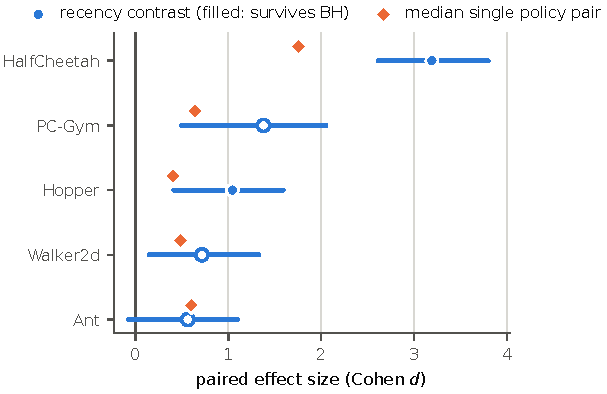
\includegraphics{figures/fig_mechanism}
\caption{Why one claim resolves and the other does not, in common effect-size
units. The paired recency contrast (circles, with 95\% intervals) is larger than
a typical single policy-versus-policy gap (diamonds) in every environment except
Ant --- the one environment where even the uncorrected contrast interval
covers zero. Filled circles
mark the contrasts that survive the exact test and multiplicity correction
(\ContrastBHList{}); open circles clear at most the uncorrected bootstrap
interval, and Ant's does not clear even that. Both quantities are paired within seed; the difference is that the
contrast aggregates three policies against five, while a ranking is decided
pair by pair.}
\label{fig:mechanism}
\end{figure}

\section{Metric disagreement needs a noise floor}
\label{sec:floor}

\paragraph{Chance is an insufficient reference.}
Permuting one metric across policies gives chance agreement, but two metrics
that are both sampling noise also cross-flip at chance. A raw flip count
therefore does not by itself demonstrate a difference in latent orderings.

\paragraph{The pair-specific estimator.}
For policy pair $j$, let $p_{Mj}$ be metric $M$'s probability of misordering
the pair on an independent half-sample, with $0\leq p_{Mj}\leq 1/2$.
Under independent half-sample errors its self-disagreement is
$f_{Mj}=2p_{Mj}(1-p_{Mj})$. Two metrics sharing a latent ordering have
concordant cross-disagreement $F_j=p_{Aj}+p_{Bj}-2p_{Aj}p_{Bj}$.
We estimate
\[
\widehat p_{Mj} =
\frac{1-\sqrt{1-2\min(\widehat f_{Mj},1/2)}}{2},
\qquad
\widehat F=\frac{1}{P}\sum_{j=1}^{P}
(\widehat p_{Aj}+\widehat p_{Bj}-2\widehat p_{Aj}\widehat p_{Bj}),
\]
and report excess $\widehat\Delta=\widehat C-\widehat F$, where
$\widehat C$ averages cross-flips of $A(h_1)$ versus $B(h_2)$ over disjoint
halves and policy pairs. Each $\widehat f_{Mj}$ is first averaged over
splits \emph{for that pair}; inversion precedes averaging over pairs.
Inverting a pooled self-rate gives a different estimator under heterogeneous
pairwise noise. Averaging the two self-rates is different again, falling
below $F_j$ by $(p_{Aj}-p_{Bj})^2$ at the population level.

At \SeedsHopper{} seeds we enumerate all \FullSplitCount{} ordered balanced
partitions of half-size \MetricHalfSize{}. Delete-one replicates enumerate
\JackSplitCount{} ordered disjoint partitions of half-size \JackHalfSize{},
leaving one seed unused per partition. This removes split Monte Carlo error;
it creates no new independent observations. The inversion assumes a
continuous latent ordering, independent identically distributed seeds and
independent half-sample errors; finite-sample self-rates may exceed one half
and are clipped, not interpreted as proof of a chance ordering.

\paragraph{Inference and calibration.}
Seed uncertainty is summarised by a leave-one-seed-out jackknife with
nominal Wald intervals and one-sided normal $p$-values. The statistic is
nonsmooth, so these are model-dependent diagnostics, not automatically valid
tests. Mistaking splits for independent evaluation units would instead
create pseudoreplication \citep{hurlbert1984pseudoreplication}.

We calibrate the \emph{same implementation} on \CalibrationCases{} Gaussian
models, each with \CalibrationDatasets{} fresh \CalibrationSeeds{}-seed
datasets: equal-noise concordance, policy-specific heterogeneous concordance,
unequal heterogeneous concordance, and a heterogeneous partial reversal.
Null type-I rates are \CalibrationRejectionEqual{},
\CalibrationRejectionHetero{} and \CalibrationRejectionUnequal{} at nominal
$\alpha=\Alpha{}$. Nominal 95\% interval coverage is
\CalibrationCoverageEqual{}, \CalibrationCoverageHetero{},
\CalibrationCoverageUnequal{} and \CalibrationCoverageReversal{},
respectively. The reversal's \CalibrationCoverageReversal{} coverage is
below the nominal target; Monte Carlo intervals and model parameters appear
in Appendix~\ref{app:calibration}. Neither these finite checks nor the largest
observed null rate proves calibration for all benchmark environments.

The table covers the four locomotion environments; the
\SeedsPcgym{}-seed reactor is excluded because its two-seed halves give a
particularly weak basis for the inversion. Update cost supplies no ranking
under the exactly equalised budget. The remaining four metrics yield
\NTests{} cells. BH flags are retained as \emph{nominal exploratory flags};
the calibration does not validate FDR control for arbitrary dependence
among the actual metrics.

\paragraph{Related metrics and updated results.}
Within a seed, \DropMetric{} is a positive affine transform of return,
because both the Frozen reference and update count are shared. Their
within-seed policy orderings match, but across-seed IQM trimming can change
aggregate rankings. Removing this related metric leaves \NDistinct{}
comparisons; they are not asserted to be independent.

The revised estimator gives \NRaw{} nominal one-sided flags before
multiplicity correction and \NBH{} nominal BH flags:
\MetricFlagDescriptions{}. Removing the improvement metric gives
\NBHDrop{} flags among the \NDistinct{} remaining comparisons:
\DropFlagDescriptions{}. All flagged cells involve drawdown-style
forgetting, the quantity defined in Section~\ref{sec:setup}; they identify
candidate metric differences rather than establish a general need for
multi-axis evaluation. Unflagged cells do not establish agreement.
In \NClamped{} of \NTests{} cells at least one policy pair is clipped
(\NClampedPairs{} of \NCellPairs{} pair-by-cell estimates), an additional
finite-sample limitation rather than saturation of every cell's mean floor.

\section{What the power diagnostic covers}
\label{sec:power}

We simulate independent Gaussian metric observations with the latent spacing
of \PowerEnv{} returns and a common noise SD of \PowerNoise{}, derived from
the observed SDs of within-seed policy differences. Reversing a growing block
of latent policy values controls the true fraction of discordant pairs.
The statistic uses the same pair-specific floor and exhaustive splits.
A threshold is the upper null quantile of \PowerDraws{} calibration draws;
each plotted point uses \PowerDraws{} \emph{independent} evaluation draws.

\begin{figure}[t]
\centering
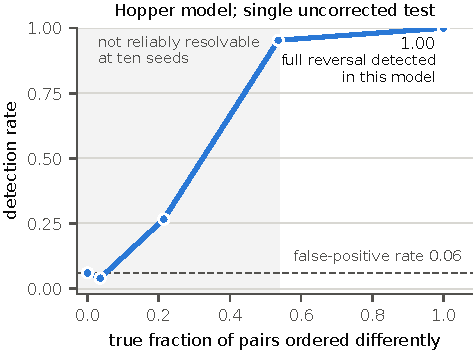
\includegraphics{figures/fig_power}
\caption{Detection in a \PowerEnv{}-derived Gaussian model at
\SeedsHopper{} seeds for a single uncorrected test. The zero-separation point
estimates false-positive rate on draws independent of threshold calibration.
The curve supplies no exclusion bound for the other environments or for
the multiplicity-corrected metric table.}
\label{fig:power}
\end{figure}

Detection is \PowerFalsePos{} at zero separation, \PowerWeakRate{} at
separation \PowerWeakSep{}, and \PowerFullReversal{} under full reversal.
The first sampled gridpoint with detection at least $0.8$ is
\PowerReliableAt{}; we do not infer an exact threshold between gridpoints.
The illustrative model is homoscedastic and covers one environment and one
uncorrected procedure. The metric table uses heterogeneous quantities,
estimated floors and BH flags, so this curve does not establish their
effective power. In particular, a non-significant cell does \emph{not}
uniformly exclude gross disagreement across the four environments.
Environment- and metric-specific power or valid inversion of tests would be
required for such a bound. No agreement or equivalence conclusion is made.

\section{What survives}
\label{sec:domain}

\paragraph{Purely recent replay reverses across environments.} A rank is not a
result, so we test the claim directly: the per-seed difference between
\textsf{RecentOnly} and the mean of the other adaptive policies, with the same
exact sign-flip test and Benjamini--Hochberg correction used elsewhere. It is
above the others on \RevAbove{} (\RoHalfcheetahMean{}, $d = \RoHalfcheetahD{}$,
positive on \RoHalfcheetahPos{} of \SeedsHalfcheetah{} seeds,
$p = \RoHalfcheetahP{}$) and below them on \RevBelow{} (\RoAntMean{},
$d = \RoAntD{}$, positive on \RoAntPos{} of \SeedsAnt{} seeds,
$p = \RoAntP{}$). Both survive correction across \RevNTests{} environments, so
the reversal is resolvable in both directions --- the only claim here that
resolves with opposite signs in different environments. Its rank-\RoHopperRank{}
position on Hopper is descriptive only ($p = \RoHopperP{}$), as is
Walker2d's ($p = \RoWalkerTwodP{}$).

Recency without an anchor is not a strategy that degrades gracefully; it is one
that inverts. We report the phenomenon rather than proposing a method to fix it,
because at this seed count we could not distinguish a proposed fix from the
policies already present.

\paragraph{``Same budget'' is definition dependent.} Update counts and replay
samples are identical across policies with zero variance. Wall-clock is not:
it spreads by \WallSpreadMin--\WallSpreadMax$\times$, grouped the same way in
every environment --- \textsf{RecentOnly} and \textsf{StaticMix} cheapest,
PER and the budgeted variants dearest --- though the full ordering permutes
within the groups. The quantity is the summed time of batch selection plus one
learner update, over every deployment update, in a single CPU process; the
grouping tracks how a policy draws its batch: \textsf{RecentOnly} and
\textsf{StaticMix} index into the buffer, while the other six ---
\textsf{Uniform} included --- score every stored transition before drawing.
A different
implementation or accelerator would move the ratio, so we read only its sign
and its grouping, not its magnitude. The direction matters at the level the surviving claim
lives at: the recency group is cheaper than the non-recency group in every
environment (\RecWallHopper{} against \NonWallHopper{} on Hopper, and
likewise elsewhere), so a wall-clock-matched budget would widen the recency
advantage rather than explain it away. \citet{korniak2026nonuniform}
report the latency profile of PER directly; the point here is narrower and about
accounting --- a benchmark that calls itself fixed-budget has fixed one resource
and left another free, and which one it picked is not neutral.

\section{Related work}

\citet{korniak2026nonuniform} is the closest study. It decomposes replay into
volume, expected recency and sampling entropy, and finds non-uniform replay most
useful when replay volume is low. Two differences matter. It studies stationary
tasks --- distribution shift appears in its future work, not its experiments ---
whereas every environment here drifts mid-deployment. And it operates at a much
lower replay volume than we do, a regime in which it predicts recency bias to be
approximately neutral; we observe a recency advantage anyway, which suggests the
mechanism under drift is staleness rather than sample efficiency. We do not
claim ``recency beats uniform'' as a finding: that is theirs, at larger scale.

Benchmarks for continual and lifelong RL, such as
\citet{wolczyk2021continualworld}, standardised the task suites and the
forgetting and transfer metrics this literature reports. Our question is
downstream of that: given such a suite, which of the comparisons it invites are
supported by the number of seeds people run on it.

On statistical practice, \citet{agarwal2021precipice} established interval
reporting and robust aggregates as the norm in RL evaluation, and
\citet{henderson2018matters} documented how far conclusions move with seeds. Our
addition is narrower: for the specific statistic of cross-metric ranking
disagreement, the reference distribution is neither zero nor chance but the
metric's own split-half noise, and once that is supplied the statistic turns out
to be underpowered at the sample sizes in use.

\section{Limitations}

This study covers four locomotion tasks at \SeedsHopper{} seeds and one reactor
at \SeedsPcgym{}; the split-half metric analysis covers only the former.
The halves are subsets of existing runs, not additional independent training
replicates. Each environment uses one shift family, and repeated events
escalate monotonically, with no return to earlier dynamics. Nothing here
establishes behaviour under recurring or cyclic shifts, different learners,
or foundation-model agents. Forgetting denotes deployment drawdown rather
than retention on an earlier task distribution.

Exact sign-flip inference requires independent seeds and a null invariant
to signs of the paired differences; label permutation requires the sharp
within-seed interchangeability null. All-pair Holm accounts for adjacent
selection but is unable to reject at this seed count. The formal
\AdjacentSeparated{}/\AdjacentTotal{} count therefore measures this
procedure's p-value resolution, not evidence that every policy comparison is
equal. The coarse contrast is a group comparison and does not identify a
preferred recency policy. Its FDR target differs from the selected-pair
audit's familywise target.

The pair-specific floor assumes independent half-sample errors around
continuous latent orderings. Finite-sample inversion, clipping and the
nonsmooth jackknife can introduce bias or undercoverage. The
\CalibrationCases{} simulation cases give \CalibrationCoverageReversal{}
coverage in the partial-reversal model at a nominal 95\%, and their
\CalibrationDatasets{} datasets each leave material Monte Carlo uncertainty.
Independent Gaussian policy/metric errors do not exhaust the benchmark's
possible dependence or heterogeneity. Consequently, the nominal Wald/BH
flags remain exploratory. The separate \PowerEnv{} power curve cannot
exclude large differences for all other metrics or environments.

The three cross-environment test families share data; joint BH across their
\JointNTests{} tests leaves the reported survivors unchanged. This sensitivity
does not validate arbitrary post-hoc hypotheses. Wall-clock comparisons
describe this implementation and hardware mix rather than a compute-optimal
policy.

\section{Conclusion}

Under identical adaptation update and replay-sample budgets, the paired
recency-group contrast survives BH in \ContrastBH{} of \ContrastNTests{}
environments, and purely recent replay reverses direction across tasks.
Selection-aware tests distinguish best from worst in \ExtremesBH{} of
\NEnv{} environments, but a complete leaderboard is not established:
all-pair Holm is resolution-limited at the observed seed counts.
Metric dependence also needs an explicit estimator and noise model.
Separately inverting each policy pair's split-half self-disagreement gives
\NBH{} nominal exploratory flags among \NTests{} metric comparisons.
Calibration exposes the estimator's finite-sample limits; a single Hopper
power curve supplies no benchmark-wide exclusion bound. These checks use
existing per-seed results, and make the scope of the evidence explicit
without inferring equality from nonrejection.

\bibliographystyle{plainnat}
\bibliography{refs}

\appendix

\section{All environment-by-metric-pair comparisons}
\label{app:cells}

Table~\ref{tab:cells} gives every cell behind Section~\ref{sec:floor}.
\emph{cross} is the flip rate between one metric on one seed half and the other
metric on the other half; \emph{floor} is the concordant rate implied by the
two metrics' separately inverted policy-pair self-disagreement over the same halves
(Section~\ref{sec:floor}). Intervals are leave-one-seed-out
jackknife Wald intervals with nominal 95\% coverage. A star marks a nominal
exploratory Benjamini--Hochberg flag at $\alpha = \Alpha{}$; neither
distribution-free interval validity nor table-wide FDR control is asserted.
Unstarred rows do not establish agreement.

\begin{table}[h]
\centering
\footnotesize
\setlength{\tabcolsep}{4pt}
\renewcommand{\arraystretch}{0.92}
\caption{Cross-metric disagreement against the mean pair-specific concordant
floor. Intervals and stars are nominal exploratory diagnostics.}
\label{tab:cells}
% Generated by scripts/export_paper_numbers.py -- do not edit by hand.
\begin{tabular}{llrrrlc}
\toprule
Environment & Metric pair & cross & floor & excess & nominal 95\% CI & \\
\midrule
ant & forgetting vs.\ improvement/1k & 0.333 & 0.383 & -0.051 & [-0.167, +0.066] &  \\
ant & recovery vs.\ forgetting & 0.377 & 0.380 & -0.004 & [-0.069, +0.061] &  \\
ant & recovery vs.\ improvement/1k & 0.238 & 0.250 & -0.012 & [-0.055, +0.031] &  \\
ant & return vs.\ forgetting & 0.336 & 0.393 & -0.057 & [-0.159, +0.045] &  \\
ant & return vs.\ improvement/1k & 0.216 & 0.200 & +0.016 & [-0.019, +0.051] &  \\
ant & return vs.\ recovery & 0.275 & 0.274 & +0.002 & [-0.028, +0.031] &  \\
halfcheetah & forgetting vs.\ improvement/1k & 0.253 & 0.303 & -0.050 & [-0.153, +0.053] &  \\
halfcheetah & recovery vs.\ forgetting & 0.410 & 0.320 & +0.090 & [+0.029, +0.150] & $\star$ \\
halfcheetah & recovery vs.\ improvement/1k & 0.222 & 0.259 & -0.037 & [-0.098, +0.024] &  \\
halfcheetah & return vs.\ forgetting & 0.247 & 0.301 & -0.054 & [-0.165, +0.058] &  \\
halfcheetah & return vs.\ improvement/1k & 0.047 & 0.045 & +0.002 & [-0.021, +0.025] &  \\
halfcheetah & return vs.\ recovery & 0.218 & 0.253 & -0.035 & [-0.107, +0.036] &  \\
hopper & forgetting vs.\ improvement/1k & 0.645 & 0.366 & +0.279 & [+0.131, +0.428] & $\star$ \\
hopper & recovery vs.\ forgetting & 0.427 & 0.446 & -0.019 & [-0.079, +0.041] &  \\
hopper & recovery vs.\ improvement/1k & 0.541 & 0.454 & +0.086 & [-0.184, +0.357] &  \\
hopper & return vs.\ forgetting & 0.635 & 0.368 & +0.267 & [+0.140, +0.395] & $\star$ \\
hopper & return vs.\ improvement/1k & 0.325 & 0.288 & +0.037 & [-0.036, +0.111] &  \\
hopper & return vs.\ recovery & 0.534 & 0.462 & +0.072 & [-0.225, +0.368] &  \\
walker2d & forgetting vs.\ improvement/1k & 0.614 & 0.402 & +0.212 & [-0.055, +0.479] &  \\
walker2d & recovery vs.\ forgetting & 0.423 & 0.406 & +0.018 & [-0.027, +0.062] &  \\
walker2d & recovery vs.\ improvement/1k & 0.535 & 0.383 & +0.152 & [-0.031, +0.335] &  \\
walker2d & return vs.\ forgetting & 0.627 & 0.377 & +0.250 & [+0.007, +0.492] &  \\
walker2d & return vs.\ improvement/1k & 0.329 & 0.297 & +0.032 & [-0.037, +0.101] &  \\
walker2d & return vs.\ recovery & 0.531 & 0.371 & +0.160 & [-0.005, +0.325] &  \\
\bottomrule
\end{tabular}

\end{table}

\clearpage
\section{Calibration design and Monte Carlo uncertainty}
\label{app:calibration}

Calibration and benchmark analysis share the implementation of the
pair-specific estimator. Each case draws
\CalibrationDatasets{} independent datasets of \CalibrationPolicies{}
policies and \CalibrationSeeds{} seeds. Latent policy means are evenly
spaced from one to zero. Equal noise uses SD \CalibrationSigma{} for both
metrics. Heterogeneous noise uses \CalibrationSigma{} times a geometric
sequence from \CalibrationSigmaLow{} to \CalibrationSigmaHigh{} across
policies, reversed for the other metric. The unequal case additionally
multiplies the second metric's SDs by \CalibrationNoiseRatio{}.
The partial reversal reverses the first half of the latent policy means.
Errors are independent across seeds, policies and metrics.

For concordant nulls the population excess is analytically zero. Coverage
is checked against zero, not against the sampling mean of a biased estimator.
For the reversal, \CalibrationPopulationDraws{} separately seeded
population half-samples approximate the target as
\CalibrationPopulationTarget{} (Monte Carlo SE
\CalibrationPopulationSE{}). Its interval coverage is checked against that
target; the small target approximation error is not included in the coverage
interval. Table~\ref{tab:calibration}'s brackets are Wilson 95\% Monte Carlo
intervals for proportions. Rejection is one-sided at $\alpha=\Alpha{}$:
type-I error for the concordant rows, power for the reversal. The cases are
fixed model checks, not tuned to produce a pass.

\begin{table}[h]
\centering
\footnotesize
\setlength{\tabcolsep}{3pt}
\caption{Finite-sample calibration of the revised estimator. Nominal interval
coverage is 95\%; rejection rate alone is not a calibration guarantee.}
\label{tab:calibration}
\begin{tabular}{lrrr}
\toprule
Model & Bias & Coverage [MC CI] & Rejection [MC CI] \\
\midrule
Equal noise, concordant & -0.010 & 0.978 [0.958, 0.988] & 0.005 [0.001, 0.018] \\
Heterogeneous, concordant & -0.000 & 0.960 [0.936, 0.975] & 0.030 [0.017, 0.052] \\
Heterogeneous, unequal & +0.028 & 0.960 [0.936, 0.975] & 0.050 [0.033, 0.076] \\
Heterogeneous, reversal & -0.002 & 0.930 [0.901, 0.951] & 0.390 [0.343, 0.439] \\
\bottomrule
\end{tabular}

\end{table}

\clearpage
\section{Training setup and reproducibility scope}
\label{app:training}

The actor and both critics are MLPs with \HiddenLayers{} hidden ReLU layers
of width \HiddenWidth{}, a squashed Gaussian actor and Adam learning rates
\ActorLR{} (actor) and \CriticLR{} (critic). SAC uses discount
\TrainGamma{}, target mixing \TrainTau{}, automatic entropy tuning with
target negative action dimension, batch size \TrainBatch{}, actor updates
when the global step is divisible by \ActorFrequency{}, and target updates
every \TargetFrequency{} global step. Random-action warmup lasts
\LearningStarts{} environment steps. Pretraining performs an update per
step once replay contains that many transitions; policy variants then share
its checkpoint and replay state within each seed. Deployment uses the
windowed update budget in Table~\ref{tab:training}. Frozen receives no
deployment updates.

Evaluation is deterministic with \EvaluationEpisodes{} episodes per
scheduled evaluation and a seed offset of \EvalSeedOffset{}; evaluation
intervals are listed in the table. Seed sets are
\TrainingSeedMinHopper--\TrainingSeedMaxHopper{} (Hopper),
\TrainingSeedMinWalkerTwod--\TrainingSeedMaxWalkerTwod{} (Walker2d),
\TrainingSeedMinAnt--\TrainingSeedMaxAnt{} (Ant),
\TrainingSeedMinHalfcheetah--\TrainingSeedMaxHalfcheetah{} (HalfCheetah), and
\TrainingSeedMinPcgym--\TrainingSeedMaxPcgym{} (reactor). Every policy in an
environment uses the same set. The observed per-run deployment updates are
\ObservedUpdatesHopper{} on Hopper, \ObservedUpdatesWalkerTwod{} on the other
locomotion tasks, and \ObservedUpdatesPcgym{} on the reactor; replay samples
equal updates times batch size.

\begin{table}[h]
\centering
\footnotesize
\setlength{\tabcolsep}{3pt}
\caption{Declared configurations, checked against observed seed grids and
update/sample budgets. Buffer/recent are transition capacities;
window/updates gives environment steps and the allowed updates per window.}
\label{tab:training}
\begin{tabular}{lrrrrr}
\toprule
Environment & Seeds & Pretrain/deploy & Buffer/recent & Window/updates & Eval interval \\
\midrule
Hopper & 10 & 50,000/70,000 & 200,000/30,000 & 2,000/1,000 & 2,000 \\
Walker2d & 10 & 60,000/90,000 & 250,000/35,000 & 2,500/1,250 & 2,500 \\
Ant & 10 & 60,000/90,000 & 250,000/35,000 & 2,500/1,250 & 2,500 \\
HalfCheetah & 10 & 60,000/90,000 & 250,000/35,000 & 2,500/1,250 & 2,500 \\
PC-Gym & 5 & 40,000/40,000 & 200,000/30,000 & 1,000/500 & 2,000 \\
\bottomrule
\end{tabular}

\end{table}

The MuJoCo source configs are \texttt{configs/train/*\_v21\_main.yaml}; the
reactor uses \texttt{configs/train/pcgym\_case\_study.yaml}, including its
normalisation, integrator, reward and constraint parameters. The small reactor
case is not evidence of general process-control behaviour. The released
per-seed CSVs suffice to reproduce analyses and manuscript artifacts without
training. Training itself requires the task simulators and additional compute;
the analysis rebuild does not establish bitwise retraining reproducibility.

\end{document}
